% This file is part of the multi-tex ECE 486 Final Project Report 
% file name: 6-extra-credit.tex

% YOU DO NOT COMPILE FROM THIS SINGLE FILE, read the following

% included files:
% (Makefile)
% Makefile -- run make Makefile (on Mac or Linux), it takes care of LaTeX compilation

% (*.PDF)
% report.pdf -- report file, print it out and submit it

% (*.TEX)
% report.tex -- main file, pdflatex this file (tested on Mac and Linux)
% 0-title-page.tex -- title page 
% 1-introduction.tex -- chapter 1 
% 2-mathematical-model.tex -- chapter 1 (lagrange equations of motion) and chapter 4 (linearisation)
% 3-full-state-feedback-control-friction-compensation.tex -- chapter 2 and chapter 4 (two state and three state feedback controller design) 
% 4-full-state-feedback-control-decoupled-observer.tex -- chapter 4 (controller design) and chapter 5 (observer design for estimated state)
% 5-conclusions.tex -- conclusion
% 6-extra-credit.tex -- (this file) (optional) add thsese pages if you have demoed chapter 6 and chapter 7

\section{Extra Credit: Up and Down Stabilizing Control}
Section 6 is about stabilizing the RWP at two different equilibrium positions. One is at the top position which is what we implemented in the previous part. The other one equilibrium point is the point at the bottom. 
Since the two equilibrium points are different, we need two sets of controllers to handle each point separately. We first linearized the system at the point $\theta_p=0$. Using the same set of pole locations. We get the controller to be [-73.5, -7.79, 0, 0.0351]. 
To switch between the two controllers, we used two conditional switches in our design to switch between the two controllers. We used the function $\cos(⁡\theta_p)$ to determine whether the pendulum is at the bottom or top positions and then switch to the corresponding controller. In addition, we also supplied two different offsets to get $\delta\theta_p$ at the two different positions. The offset is $\pi$ at the top position and is 0 at the bottom position.

\begin{figure}
  \caption{Our control block diagram of our Up-Down Control}
  \centering
    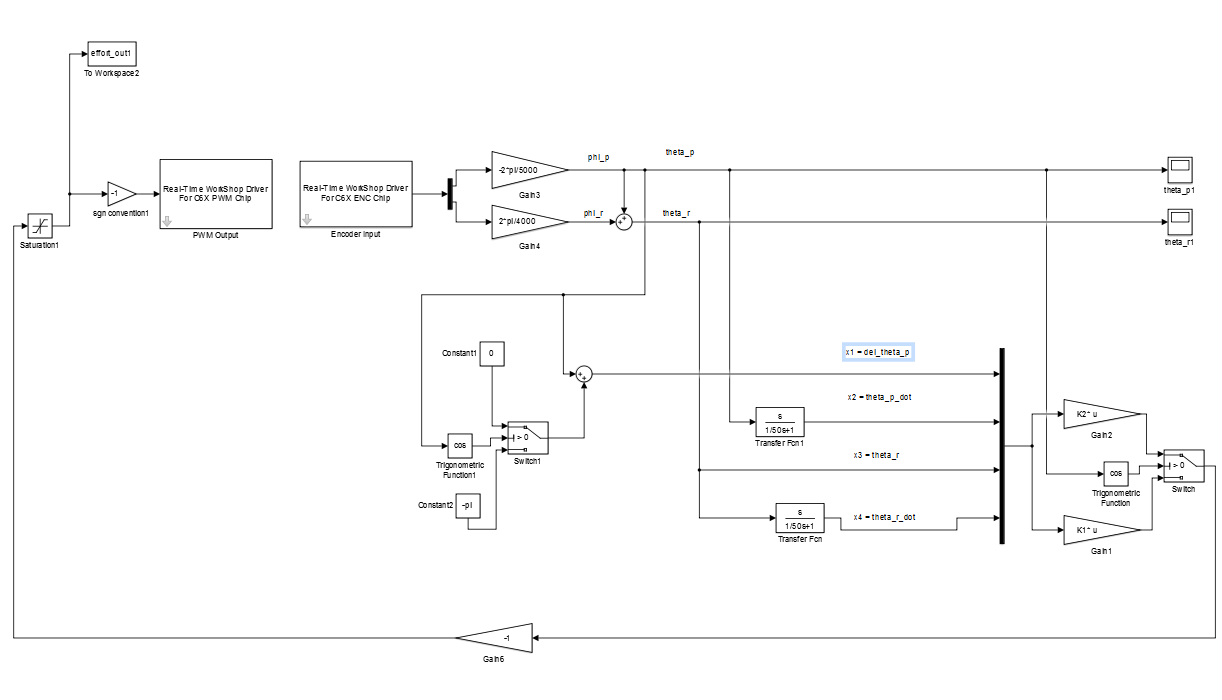
\includegraphics[scale = 0.4]{updown.PNG}
\end{figure}

\section{Extra Credit: Swing-Up Control}
We implemented section 7 by supplying forces along the direction of the swing of the pendulum to make it swing up to the equilibrium position.
In this section, we used 5 conditional switches to implement the swing-up controllers. The first conditional switch is used to switch between two situations where the pendulum is at left or right to the mount. For each situation, we have two switches. The conditions to the two switches are the angular velocities of the pendulum. When the angular velocities start to change sign, i.e. the pendulum has reached its maximum height in one swing, we supply a constant force along the direction to increase its kinetic energy. The other switch is used to handle the situation of overshoot. When the pendulum is swinging too fast – in the case we manually pushed the pendulum down from the top positions – the switch will switch to supplying no force so that the pendulum will be slowed and then return to the equilibrium position. With some trials, we determined that the best force to supply to our pendulum is 5 which will ensure a rather smooth swing to the top position.

\begin{figure}
  \caption{Our control block diagram of our Swing-Up Control}
  \centering
    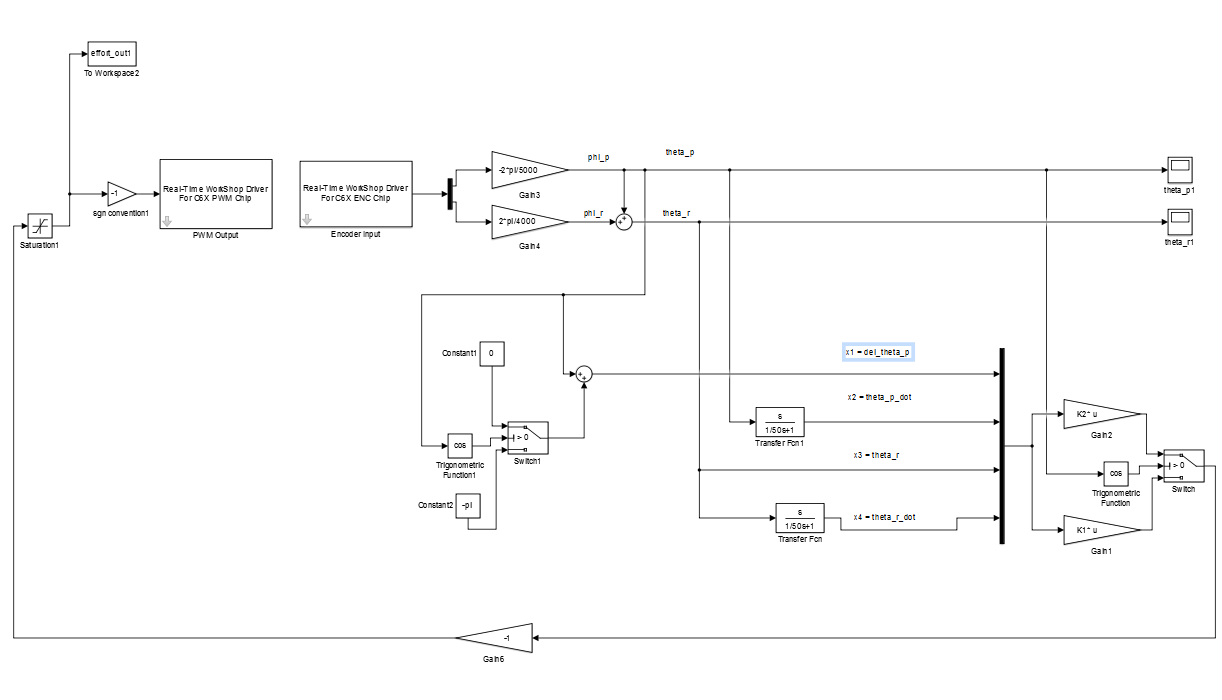
\includegraphics[scale = 0.4]{updown.PNG}
\end{figure}